\documentclass[12pt]{article}
\usepackage[margin=1in]{geometry}
\usepackage{amsmath}
\usepackage{tcolorbox}
\usepackage{float}
\usepackage{amssymb}
\usepackage{amsthm}
\usepackage{lastpage}
\usepackage{fancyhdr}
\usepackage{accents}
\pagestyle{fancy}
\setlength{\headheight}{40pt}
\usepackage[utf8]{inputenc}
\title{The Math of Ray Tracing}
\author{Ramy Kaddouri \\ Centennial High School Junior}
\date{}

\begin{document}

\maketitle

\section{Introduction}
    Ray tracing is a technique for generating 3D computer graphics that attempts to simulate the behavior of light in real life. Due to its ability to accurately model light transport, ray tracing is widely used in animated movies and VFX to generate photorealistic images. Recent advances in hardware acceleration have made ray tracing a viable alternative to rasterized rendering for games and other performance sensitive tasks. Since its inception in 1971, it remains one of the simplest and most intuitive ways to generate 3D images and serves as a classic introduction to the mathematical foundations of computer graphics.
\begin{figure}[h]
    \centering
    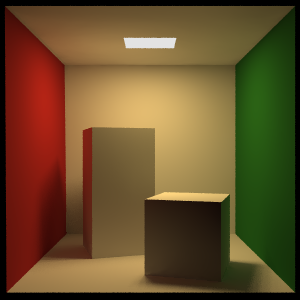
\includegraphics[scale=0.7]{figures/Cornell_box.png}
    \caption{The Cornell Box, a commonly used test scene for ray tracers showcasing indirect lighting capabilities (Wikimedia Commons)}
    \label{fig:cornell_box}
\end{figure}
\\
\noindent
This article will be fairly light on implementation details, focusing more on the theory of ray tracing. Nonetheless, the information should be sufficient to implement your own basic ray tracer in a language of your choice with simple shading, shadows, and reflections.
\section{A Simple Camera and Rays}
    \subsection{Defining the Virtual Camera}
        To begin rendering a scene, we must first establish our viewpoint, often represented by a virtual camera. We can define the camera using the following parameters: 
$$\Vec{P} \text{ is a three dimensional vector representing the camera's position}$$
$$\hat{V} \text{ is a \textbf{normalized} three dimensional vector representing the camera's direction}$$
$$ w \text{ is the viewport width} $$
$$ h \text{ is the viewport height} $$
$$ z \text{ is the distance of the viewport's near plane from the position along $\hat{V}$}$$

\begin{tcolorbox}
   \textbf{Note:} all three dimensional vectors relating to position or direction will be in the form $\begin{bmatrix} x \\ y \\ z \end{bmatrix}$ unless otherwise specified.
\end{tcolorbox}

\begin{figure}[h]
    \centering
    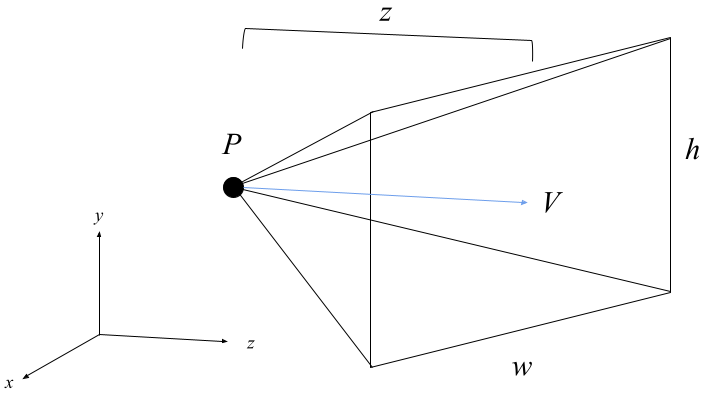
\includegraphics[scale=0.4]{figures/CameraDefinition.png}
    \caption{Visualization of the camera definition}
    \label{fig:camera_def}
\end{figure}
    \subsection{Rendering Approach}
        \noindent
Having established our viewport, we must now determine how to render the scene. In the real world, light sources cast light which subsequently interacts with nearby objects. Certain components of the light are then reflected or absorbed by the object based on its material properties. Eventually, some of the light will hit our eyes or the sensor of a camera, producing an image.
\begin{figure}[H]
    \centering
    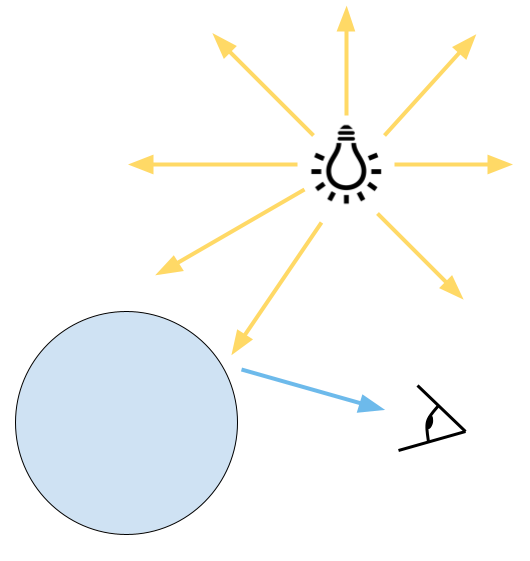
\includegraphics[scale=0.3]{figures/ForwardRT.png}
    \caption{Scene with a single point light and sphere. Note that the viewport captures a limited amount of all light in the scene.}
    \label{fig:forward_rt}
\end{figure}

\noindent
Directly simulating this process is inefficient as only a small fraction of the light produced in the scene will hit the camera. Instead, we can perform the reverse, by casting rays from the camera's viewport and determining how they subsequently interact with the scene and light sources in order to produce an image from the camera's perspective.
    \subsection{Camera Rays}
        We can define a ray as having two components:
$$\Vec{O} \text{ a three dimensional vector representing the ray's origin}$$
$$\text{and}$$
$$\hat{D} \text{ a \textbf{normalized} three dimensional vector representing the ray's direction}$$
These two components can be combined to provide a unified definition:
$$ \Vec{O} + t\hat{D} $$
where $t$ is a scalar which represents a distance along the ray's direction from the origin. \\ \\
\noindent
To render a scene, we must cast at a ray for each pixel on the screen in order to determine the pixel's color. The ray's origin will be defined as the camera's position while the ray's direction must be calculated by mapping pixel coordinates on to the camera's viewport. First we can define our screen dimensions with $S_w$ being the screen's width in pixels and $S_h$ being the screen's height in pixels. Considering that the orientation of the camera's viewport will be determined by the camera's direction, we can find the relative horizontal and vertical unit vectors of the viewport ($\hat{H}$ and $\hat{U}$ respectively) using vector cross products as follows:

$$\hat{H} = \begin{bmatrix} 0 \\ 1 \\ 0 \end{bmatrix} \times \hat{V}  $$
$$\hat{U} = \hat{H} \times \hat{V}$$

\noindent
For example, if the camera direction $\hat{V}$ is $\begin{bmatrix} 0 \\ 0 \\ 1 \end{bmatrix}$, then $\hat{H}$ will be $\begin{bmatrix} 1 \\ 0 \\ 0 \end{bmatrix}$ and $\hat{U}$ will be $\begin{bmatrix} 0 \\ 1 \\ 0 \end{bmatrix}$

\noindent
Based on these vectors, we can begin calculating the direction and origin of our camera ray's. First, we know that $\Vec{O} = \Vec{P}$ because all camera rays will originate from the camera's position. Next, we can calculate the bottom left corner of our viewport in world space as
$$\Vec{B} = -\frac{w}{2}\hat{H} - \frac{h}{2}\hat{U}$$
Given a screen pixel coordinate ($x$, $y$), we are now ready to determine the corresponding camera ray's direction.
$$\Vec{A} = \Vec{B} + (w \frac{x}{S_w})\hat{H} + (h \frac{y}{S_h})\hat{U} + z\hat{V}$$
Normalizing $\Vec{A}$ gives us our final direction:
$$\hat{D} = \frac{\Vec{A}}{|\Vec{A}|} = \frac{\Vec{B} + (w \frac{x}{S_w})\hat{H} + (h \frac{y}{S_h})\hat{U} + z\hat{V}}{|\Vec{B} + (w \frac{x}{S_w})\hat{H} + (h \frac{y}{S_h})\hat{U} + z\hat{V}|}$$
Now, we can define our camera ray for a particular pixel ($x$, $y$) as:
$$R = \Vec{P} + t(\frac{\Vec{B} + (w \frac{x}{S_w})\hat{H} + (h \frac{y}{S_h})\hat{U} + z\hat{V}}{|\Vec{B} + (w \frac{x}{S_w})\hat{H} + (h \frac{y}{S_h})\hat{U} + z\hat{V}|})$$

\begin{figure}[H]
    \centering
    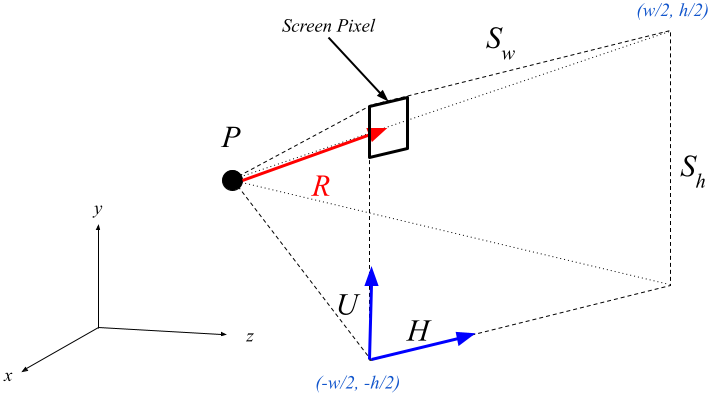
\includegraphics[scale=0.5]{figures/CameraRays.png}
    \caption{Diagram of ray generation and mapping from screen to viewport space. Pixel's near the center of the screen will have fairly straight corresponding camera rays while pixels near the corners will have angled camera rays, simulating distortion in the camera's peripheral vision.}
    \label{fig:cam_rays}
\end{figure}
\noindent
To begin generating an image, we must calculate the corresponding ray for each pixel and trace its path in the scene over time as demonstrated in the illustration below.

\begin{figure}[H]
    \centering
    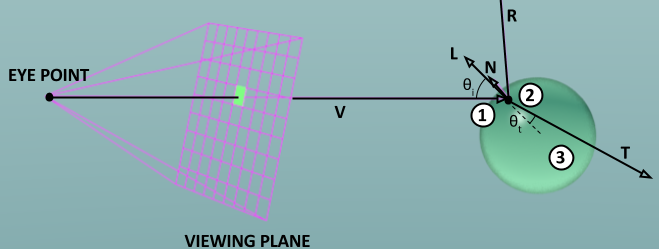
\includegraphics[scale=0.5]{figures/ApproachIllustration.png}
    \caption{Process of determining pixel color based on the interactions of camera ray $v$ with the scene (Wikimedia Commons)}
    \label{fig:approach}
\end{figure}
\noindent
For now, given that we have yet to define any scene objects, we will assign a color, represented by a three dimensional vector in the form $\begin{bmatrix}\text{red}, \text{green}, \text{blue} \end{bmatrix}$ where each component ranges from 0 to 1, to each pixel based on the $y$ component of the pixel's corresponding camera ray direction. When placing the camera at the point $\begin{bmatrix}0, 0, -1 \end{bmatrix}$ with direction $\begin{bmatrix}0,  0, 1 \end{bmatrix}$, $z = 1$, and $h = 2, w = 2\frac{16}{9}$ (the standard 16:9 aspect ratio), this produces the following image when giving higher $y$ components a darker blue color and lower $y$ components a lighter blue color in order to simulate the appearance of a clear sky.

\begin{figure}[H]
    \centering
    
\includegraphics[scale=0.4]{figures/FirstImage.png}
    \caption{First image generated by varying each pixel's color based on the $y$ component of the pixel's corresponding camera ray's direction.}
    \label{fig:first_image}
\end{figure}
\section{Drawing a Sphere}
    Now that we have a camera and a method for generating camera rays, we can begin rendering scene objects. One of the simplest primitives to draw using a ray tracer is a sphere which can be defined as follows:
$$(\Vec{S} - \Vec{P})^2 = r^2$$
\begin{tcolorbox}
\textbf{Note:} Vector multiplications in the following equations should be treated as dot products returning a scalar value.
\end{tcolorbox}
\noindent
Where $\Vec{S}$ represents a point on the sphere's surface in the form $\begin{bmatrix} x, y, z \end{bmatrix}$, $\Vec{P}$ represents the origin of the sphere in the same form as $\Vec{S}$, and $r$ represents the sphere's radius. Given a sphere and a ray, our goal is to find their point(s) of intersection. Recall our earlier definition of a ray as $\Vec{O} + t\hat{D}$ where $\Vec{O}$ is the ray's origin, $\hat{D}$ is the ray's direction, and $t$ is a distance along $\hat{D}$ from the ray's origin. This can be substituted for $\Vec{S}$ in the sphere definition to get the following:
$$(\Vec{O} + t\hat{D} - \Vec{P})^2 = r^2$$
Solving for $t$ in the above equation will yield the distance(s) along the ray where it intersects the sphere.
\begin{align*}
    &\Vec{O}^2 + \Vec{O}t\hat{D} - \Vec{O}\Vec{P} + \Vec{O}t\hat{D}  + t^2\hat{D}^2 - t\hat{D}\Vec{P} - \Vec{O}\Vec{P} - \Vec{P}t\hat{D} + \Vec{P}^2 = r^2 &\text{expand left side}&\\
    &\Vec{O}^2 + \Vec{P}^2 - 2\Vec{O}\Vec{P}  - r^2 + 2\Vec{O}\hat{D}t - 2\hat{D}\Vec{P}t + \hat{D}^2t^2 = 0 &\text{combine terms and move $r^2$}&\\
    &\hat{D}^2t^2 + (2\Vec{O}\hat{D}-2\hat{D}\Vec{P})t + \Vec{O}^2 + \Vec{P}^2 - 2\Vec{O}\Vec{P} - r^2 = 0 &\text{rearrange terms}&
\end{align*}
Notice that the equation above is a quadratic in the form $at^2 + bt + c = 0$ where 
\begin{align*}
    a &= \hat{D}^2 &&= 1 \\
    b &= 2\Vec{O}\hat{D}-2\hat{D}\Vec{P} &&= 2\hat{D}(\Vec{O}-\Vec{P}) \\
    c &= \Vec{O}^2 + \Vec{P}^2 - 2\Vec{O}\Vec{P} - r^2 &&= (\Vec{O}-\Vec{P})^2-r^2
\end{align*}
Therefore, we can attempt solving using the quadratic formula:
$$
t = \frac{-2\hat{D}(\Vec{O}-\Vec{P}) \pm \sqrt{(2\hat{D}(\Vec{O}-\Vec{P}))^2 - 4((\Vec{O}-\Vec{P})^2-r^2)}}{2}
$$
Like with any other quadratic, we can use the discriminant, in this case $d = (2\hat{D}(\Vec{O}-\Vec{P}))^2 - 4((\Vec{O}-\Vec{P})^2-r^2)$, to make conclusions about the number of solutions:
\begin{enumerate}
    \item $d < 0$: There are no intersection points between the ray and the sphere
    \item $d = 0$: There is exactly one intersection point between the ray and the sphere
    \item $d > 0$: There are exactly 2 intersection points between the ray and the sphere
\end{enumerate}
If we have at least one solution, we can obtain more information based on the value(s) of $t$:
\begin{enumerate}
    \item $t < 0$: The intersection point is behind the camera and is not visible
    \item $t \geq 0$: The intersection point is at or in front of the camera's position and is visible
\end{enumerate}
For now, to quickly visualize the sphere, we will fill pixels whose corresponding camera ray's have intersection(s) with the sphere at $t \geq 0$ with a solid green color. When we have two points of intersection, we will only use the one with a lower $t$ in order to only render the camera facing part of the sphere while ignoring the back. Placing a sphere at the point $\begin{bmatrix} 0, 0, 1 \end{bmatrix}$ with radius $r = 1$ and a camera at $\begin{bmatrix} 0, 0, -1 \end{bmatrix}$ with direction $\begin{bmatrix} 0, 0, 1 \end{bmatrix}$ and the same viewport dimensions as earlier, we get the following image:

\begin{figure}[H]
    \centering
    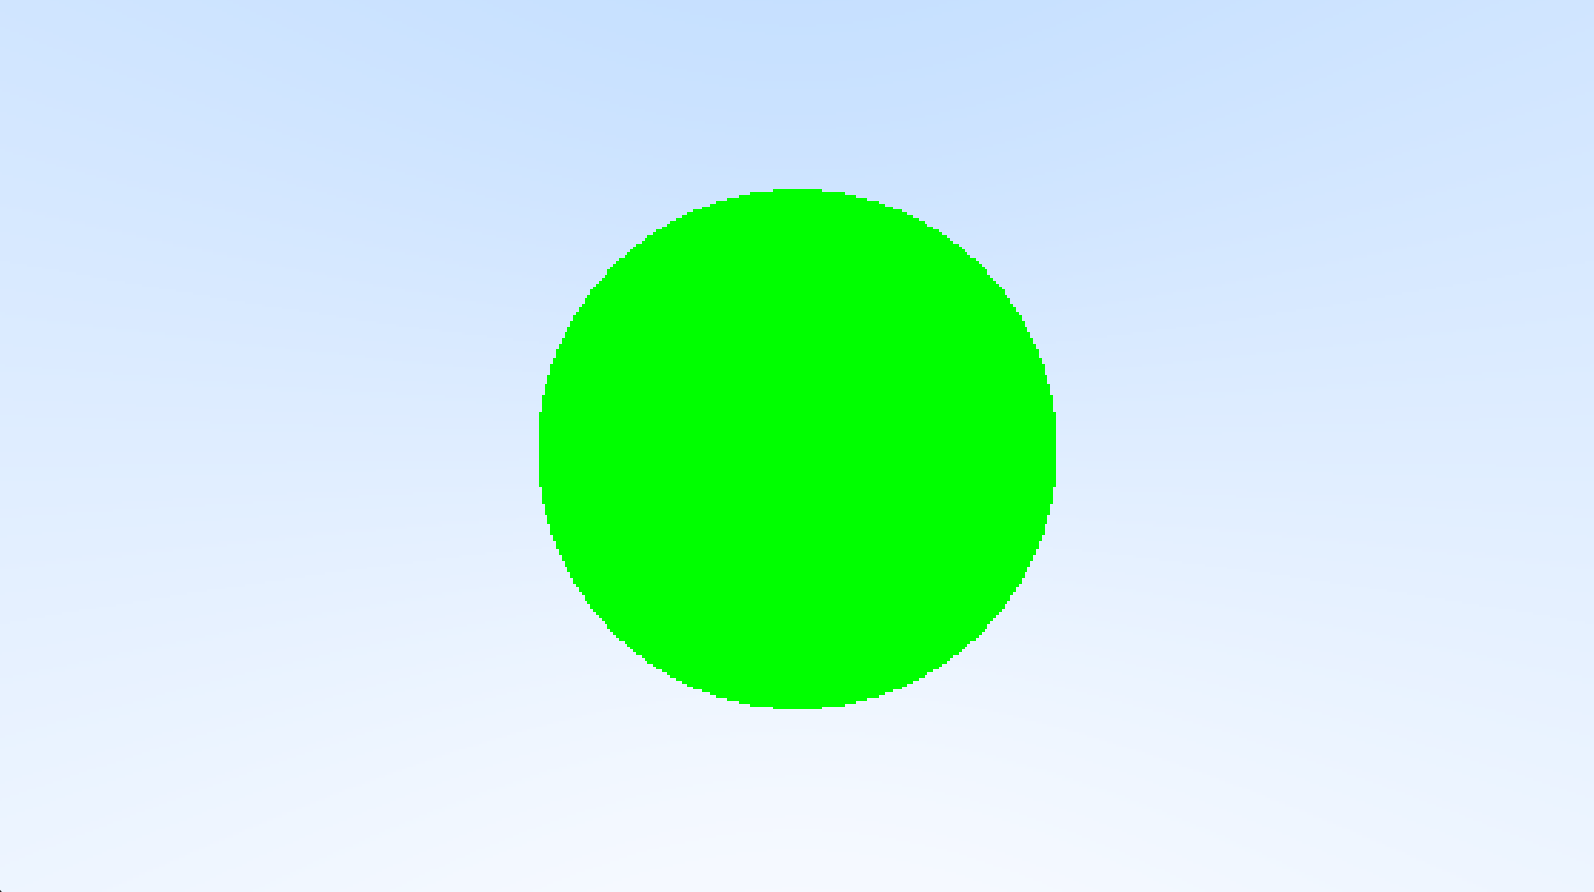
\includegraphics[scale=0.5]{figures/GreenSphere.png}
    \caption{Sphere rendered without shading}
    \label{fig:green_sphere}
\end{figure}
\noindent
Of course, the rendered image above looks more like a circle than a sphere because we have yet to introduce lighting and shading. A key piece of information we need for lighting calculations is the sphere's normal at a point on its surface. The surface normal, $\hat{N}$, can be thought of as a normalized three dimensional vector that is perpendicular to the sphere's surface. 
\begin{figure}[H]
    \centering
    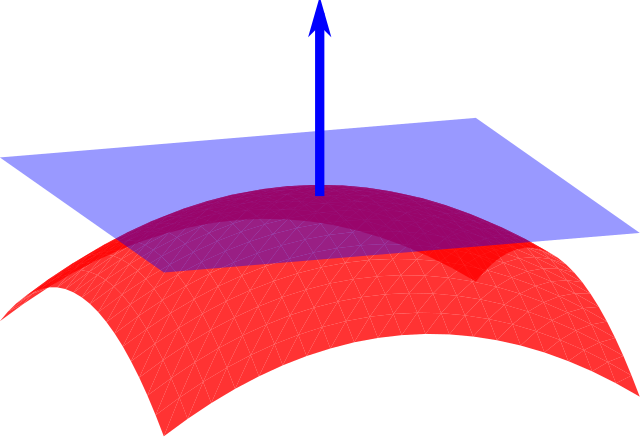
\includegraphics[scale=0.3]{figures/normal.png}
    \caption{Illustration of a surface normal (blue arrow) (Wikimedia Commons)}
    \label{fig:normal_example}
\end{figure}
\noindent
Given a point of intersection $\Vec{I}$ and the center of the sphere $\Vec{P}$, we can calculate the normal as follows:
$$\hat{N} = \frac{\Vec{I} - \Vec{P}}{|\Vec{I} - \Vec{P}|}$$
\begin{tcolorbox}
\textbf{Note:} Given that we have solved for $t$, finding the point of intersection simply involves substituting the value of $t$ into the definition of a ray $\Vec{O} + t\hat{D}$.
\end{tcolorbox}
\noindent
To visualize this, we can assign colors based on the surface normal at each intersection point with the following mapping:
$$\text{Color} = \frac{\hat{N} + \begin{bmatrix} 1\\ 1\\ 1 \end{bmatrix}}{2}$$
This yields the following image of our earlier sphere:
\begin{figure}[H]
    \centering
    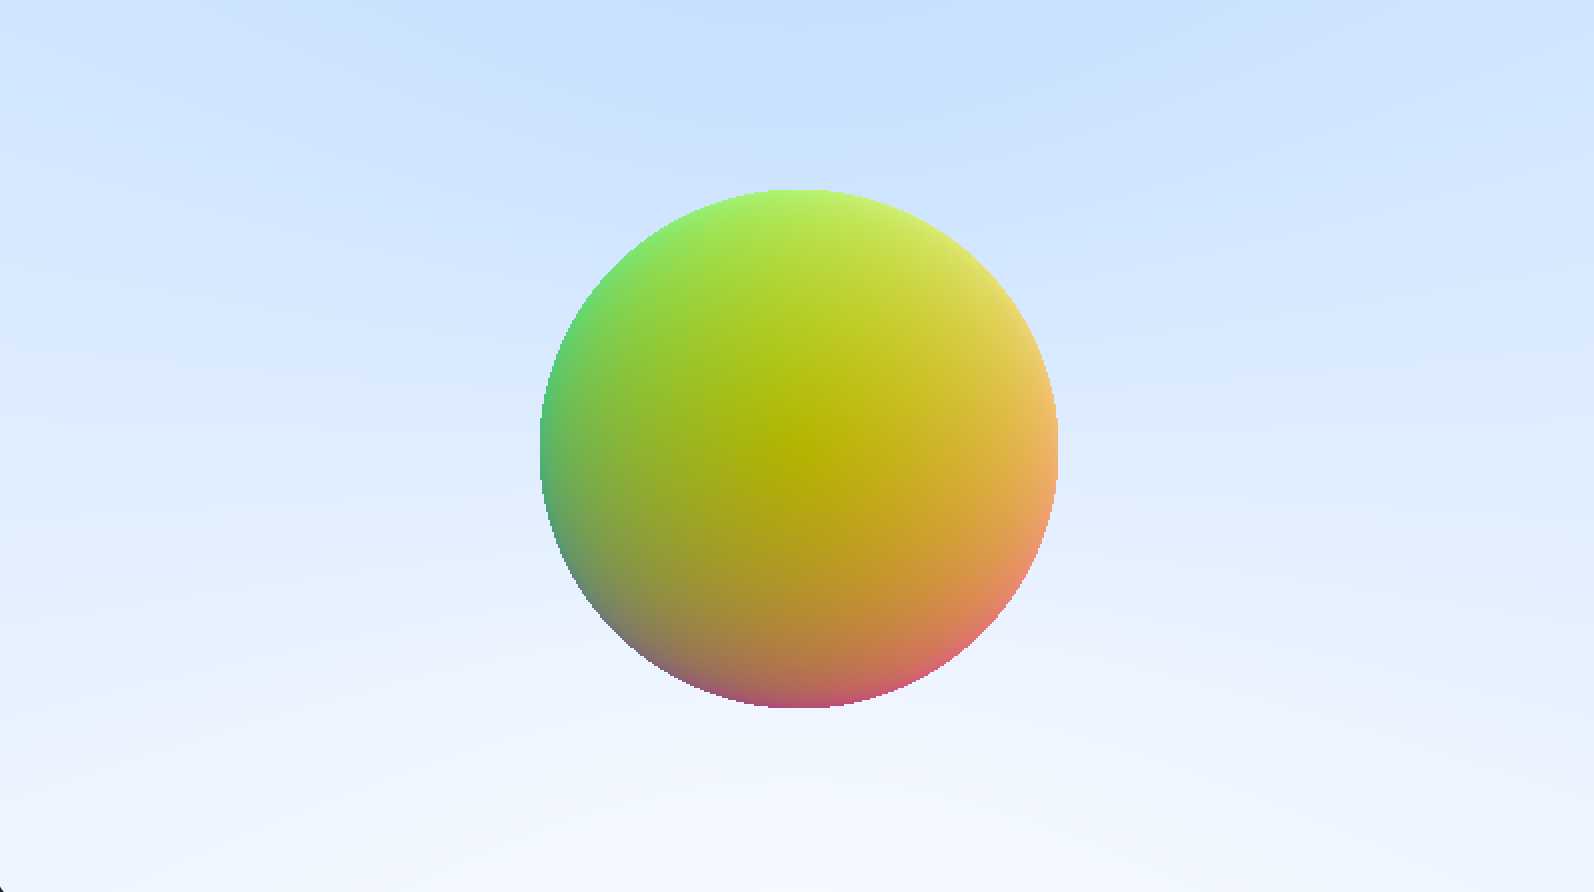
\includegraphics[scale=0.5]{figures/SphereNormal.png}
    \caption{Sphere visualized with surface normals}
    \label{fig:sphere_normal}
\end{figure}
\section{Basic Lighting, Shadows, and Reflections}
    \subsection{Lighting}
        To begin implementing lighting, we must first establish a light source in the form of a directional light. Directional light sources uniformly light objects in the scene from one direction, similar to how the sun illuminates objects on Earth. We can define a directional light using two parameters:
$$ \hat{L} \text{ a \textbf{normalized} three dimensional vector representing the direction of the light}$$
$$ \Vec{I} \text{ a three dimensional color vector representing the intensity of the light}$$
For shading, we will use a modified Phong shading model only including the ambient and diffuse lighting components:
$$
\text{Color} = \Vec{K}a + \sum_{n \in \text{lights}}(\Vec{K}\Vec{I}_{n}(\hat{L}_{n} \cdot \hat{N}))
$$
Where $\Vec{K}$ is three dimensional vector representing the color of the object, $a$ is the ambient lighting coefficient ($0 \leq a < 1$), $\hat{L}_n$ is the direction of light $n$, $I_n$ is the intensity of light $n$, and $\hat{N}$ is the surface normal of the object. Note that the multiplication of $\Vec{K}$ and $\Vec{I}_n$ is a component-wise product. To better understand what this equation is doing, we can break it up into parts, beginning with the ambient component.
$$\Vec{K}a$$
In the real world, objects usually receive some indirect lighting from their surroundings even when they are in shadow or when there is no direct light source present. The ambient component accounts for this by allowing for slight illumination of unlit surfaces. Since $a$, the ambient lighting coefficient, is always less than 1, ambient lighting will naturally be less than lighting from direct light sources, ensuring that unlit areas will appear darker than areas in direct light. Next, we can take a look at the diffuse lighting component.
$$\Vec{K}\Vec{I}_{n}((-\hat{L}_{n}) \cdot \hat{N})$$
Diffuse shading aims to model the appearance of rough, non-reflective surfaces like paper. The dot product between $-\hat{L}_{n}$ and $\hat{N}$, both normalized vectors, essentially acts as a measure of similarity of the light direction and surface normal. If the surface normal and light direction are pointing directly towards each other (light is pointing towards the surface), this value will be 1, 0 if perpendicular, and -1 if pointing in the same direction (light is pointing away from the surface). This is very useful for lighting calculations as we only want to illuminate surfaces that are facing the light source. Therefore, if the result of the dot product is less than 0, we know that the surface should receive no light from light source $n$. If the result is greater than zero, we scale the intensity of light source $n$, $\Vec{I}_n$, by the result. Finally, we perform a component-wise multiplication of $\Vec{K}$ and $\Vec{I_n}$ to obtain our final diffuse lighting component. Note that in the full equation, this component is summed over all light sources in the scene and then added to the ambient component to get the final color for a specific pixel. Implementing lighting into our earlier scene configuration with a white sphere and a directional light pointing in the direction $\begin{bmatrix}-1, -1, 1\end{bmatrix}$ (Automatically normalized in the actual implementation) with a uniform intensity of $\begin{bmatrix}1, 1, 1\end{bmatrix}$ gives us the following image:
\begin{figure}[H]
    \centering
    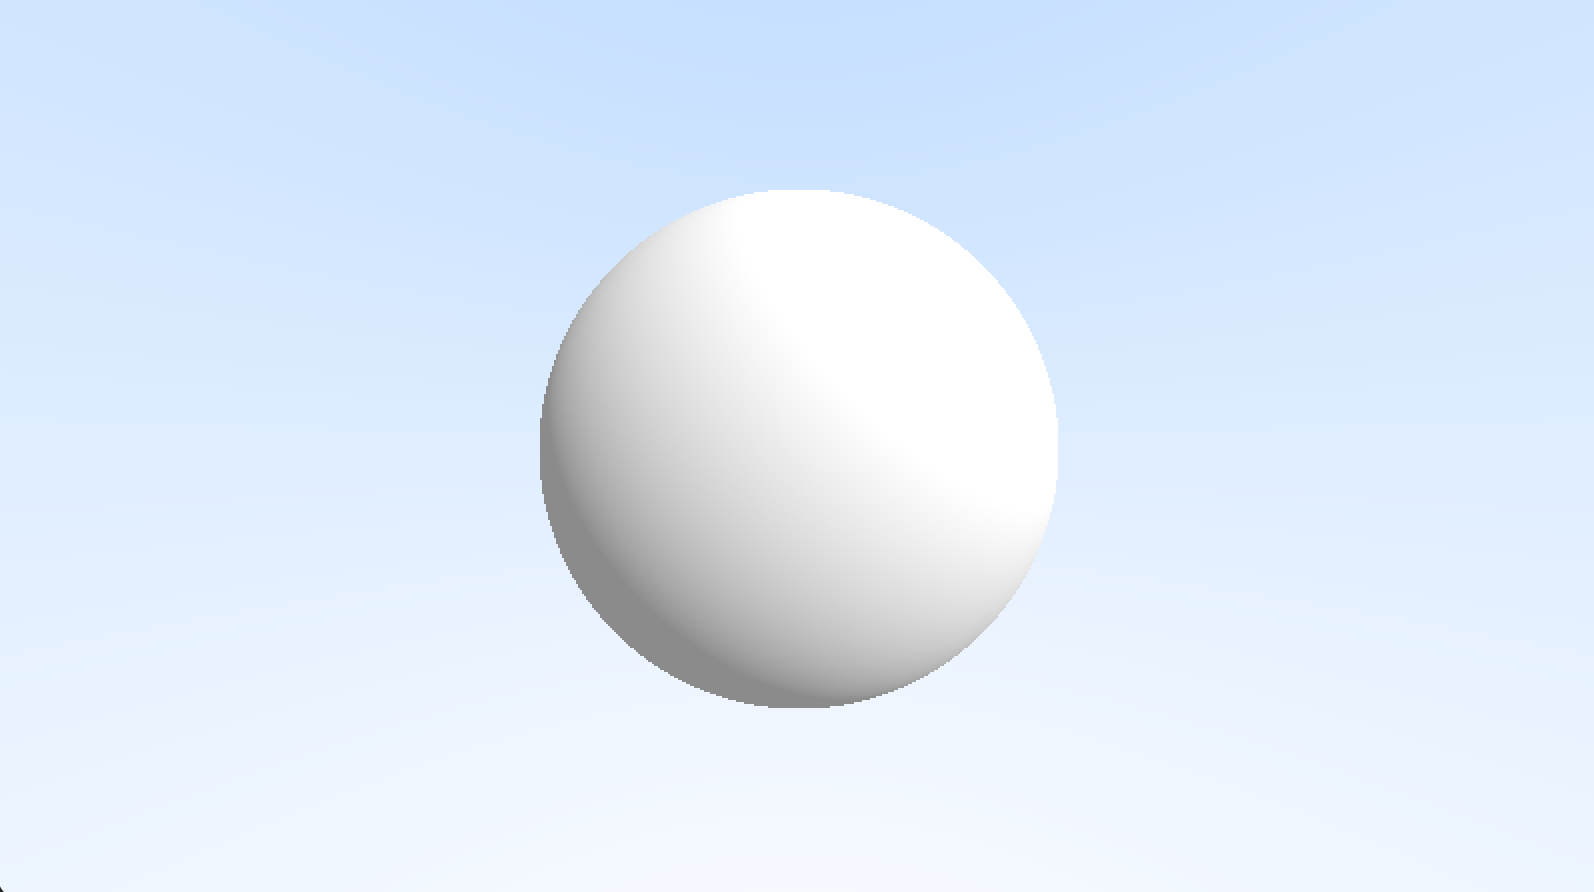
\includegraphics[scale=0.4]{figures/DiffuseSphere.png}
    \caption{Sphere with diffuse shading from a directional light}
    \label{fig:diffuse_sphere}
\end{figure}
    \subsection{Shadows}
        Shadows are the result of an surface being occluded from a direct light source by another object in the scene. To determine whether this is the case, we can define a shadow ray $S$ as follows:
$$S = \Vec{P} - t\hat{L}_n$$
Where $\Vec{P}$ is a point of intersection on a scene object and $\hat{L}_n$ is the direction of light source $n$. Note that $t\hat{L}_n$ is being subtracted from the ray's origin as the shadow ray should point towards the light source from the point of intersection.
\begin{figure}[H]
    \centering
    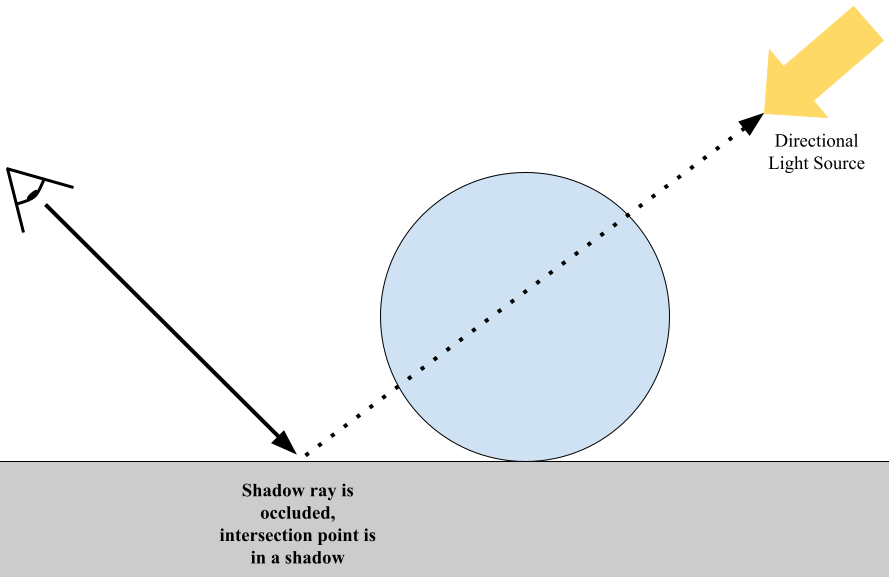
\includegraphics[scale=0.4]{figures/Shadows.png}
    \caption{Diagram of shadow rays}
    \label{fig:shadow_diag}
\end{figure}
\noindent
To determine whether the intersection point is in a shadow or not, we must simply cast the shadow ray into the scene and check for intersections with other scene objects. If an intersection is found, then the intersection point is in a shadow and should only receive ambient lighting. If not, then the intersection point is illuminated by a light source and should receive both ambient and diffuse lighting components. Implementing this logic gives us the following image when adding another, much larger sphere with a different color underneath our original.
\begin{figure}[H]
    \centering
    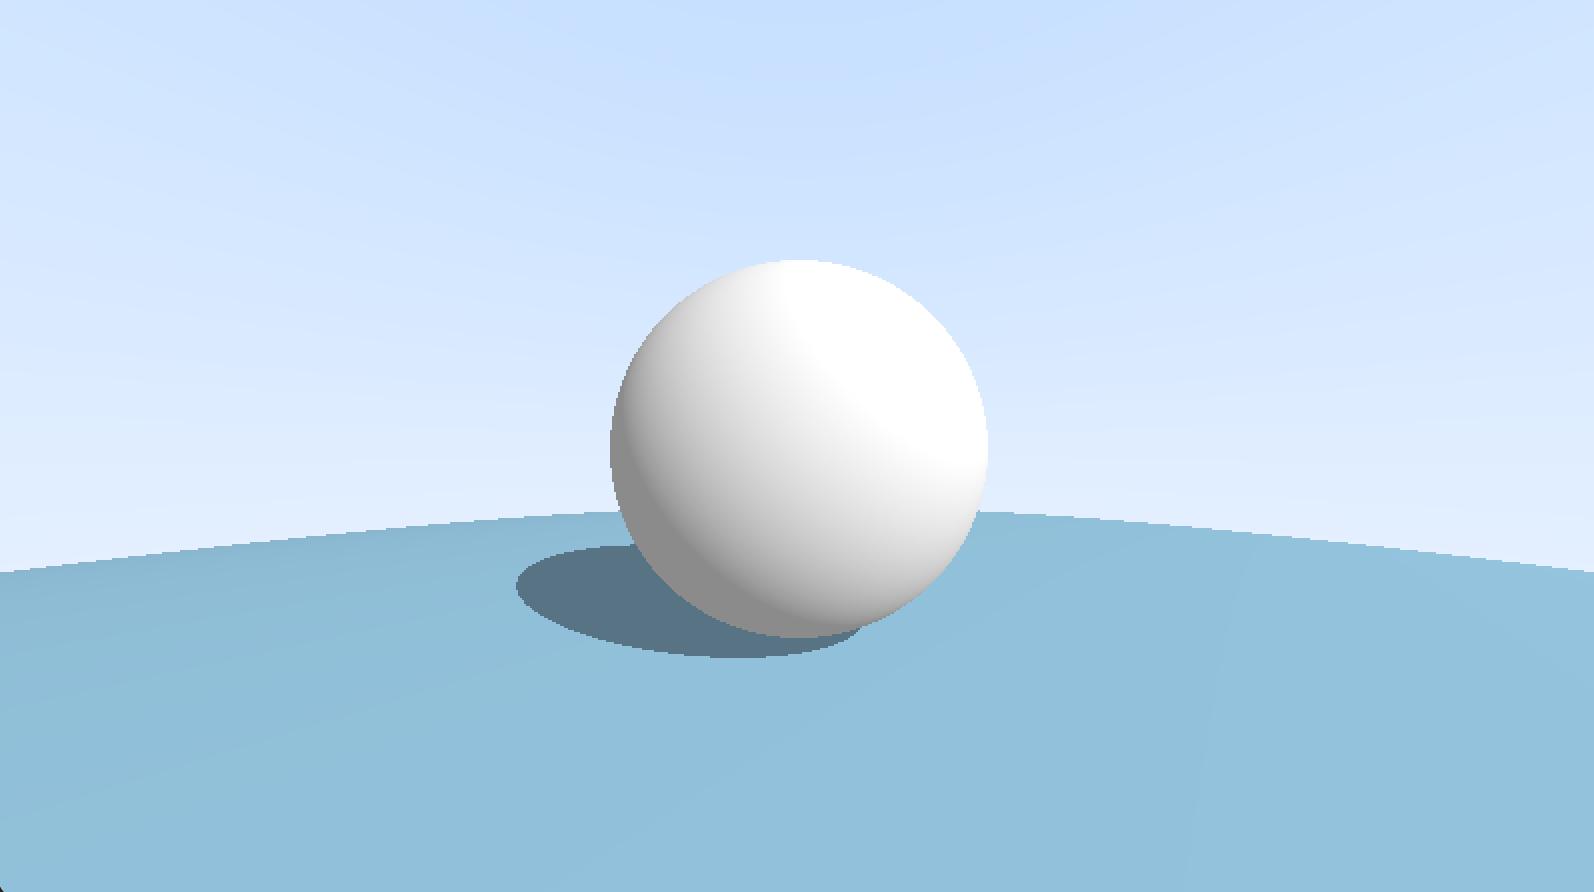
\includegraphics[scale=0.5]{figures/SphereShadows.png}
    \caption{A scene with two spheres to demonstrate shadows}
    \label{fig:sphere_shadows}
\end{figure}
\noindent
You may notice that the shadow illustrated in the image above ends abruptly, unlike shadows in the real world which are much softer. This is because points on the surfaces of objects can be partly occluded from light sources, creating a \textit{penumbra}, or soft shadow, which is not accounted for in this implementation. However, this effect can be achieved in a ray tracer by casting many shadow rays, each with slight randomness added to their direction, and averaging whether they are occluded or not, adjusting the strength of the shadow accordingly.
    \subsection{Reflections}
        Reflections are one of the distinguishing features of ray tracers, setting them apart from other methods of 3D rendering. When a ray of light hits a perfect reflective surface, like a mirror, the ray is reflected along the surface normal.
\begin{figure}[H]
    \centering
    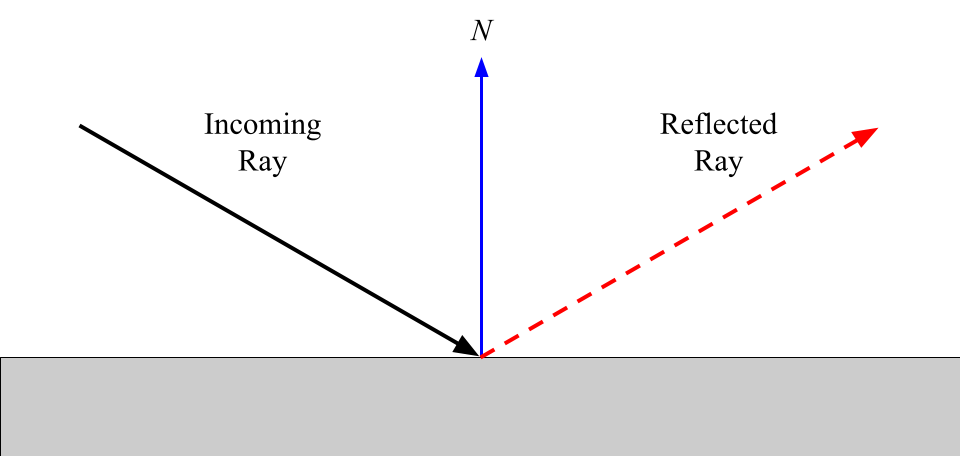
\includegraphics[scale=0.35]{figures/Reflections.png}
    \caption{Result of reflecting a ray over a surface normal}
    \label{fig:reflection_ray}
\end{figure}
\noindent
We can calculate the result of reflecting a ray over a surface normal, $\hat N$ as follows:
$$R = \Vec{P} + t(\hat{D} - 2(\hat{N} \cdot \hat{D})\hat{N})$$
Where $\Vec{P}$ is the intersection point of the incoming ray and the surface and $\hat{D}$ is the direction of the incoming ray. Now, it is important to remember that our rendering approach is the reverse of how light behaves in reality (See 2.2). Given this, we must also approach reflections in the same way. For example, if a camera ray intersects a perfectly reflective sphere, in order to determine the color of the sphere at that point, we must cast the corresponding reflection ray into the scene. There are three different possibilities for how this ray will subsequently behave:
\begin{enumerate}
    \item The reflection ray does not intersect any other object. In this case, the color of the sphere at the intersection point with the camera ray should be the same as the sky color calculated using the reflected ray's $y$ component.
    \item The reflection ray intersects a diffusely shaded, non-reflective object. In this case, the color of the sphere at the intersection point with the camera ray should be the same as the color of the non-reflective object at the intersection point with the reflected ray.
    \item The reflection ray intersects another reflective object. In this case we must recursively cast another reflection ray and compute our final color based on its resulting interactions with the scene.
\end{enumerate}
Note that the third possibility is a recursive case, meaning that when the first reflected ray is cast, we must perform the same calculations on it as the original camera ray. This presents the chance of an infinite recursion depth when reflection rays keep bouncing between adjacent reflective objects, often seen in real life when having two mirrors pointing at each other. This is usually solved by enforcing a maximum amount of light bounces and ignoring reflections beyond the maximum. So far, we have only discussed perfect reflective surfaces. However most objects are not perfectly reflective. We can account for this by defining a shininess coefficient $s$ where $0 \leq s \leq 1$ and $s = 1$ is a perfectly reflective surface while $s = 0$ is a diffuse, non-reflective surface. This allows us to define pixel color as follows by assigning diffuse and reflective shading different weights based on $s$:
$$\text{Color} = (1-s)\Vec{d} + s(\Vec{d}\Vec{r})$$
Where $\Vec{d}$ is a three dimensional color vector representing result of the diffuse lighting calculations discussed earlier and $\Vec{r}$ is a three dimensional color vector representing the color returned from the reflected ray, including subsequent recursive reflections which will employ the same shading equation. Note that the product of $\Vec{d}$ and $\Vec{r}$ is another color vector which is the result of a component-wise multiplication.
\\
\\
\noindent
To demonstrate reflections, we can create a scene with multiple reflective objects to see how they interact. The following image includes 9 spheres with random colors and a shininess coefficient of 0.8, a plane with a checkerboard pattern and a shininess coefficient of 0.3, and a directional light:
\begin{tcolorbox}
\textbf{Note: }Ray-plane intersection was not discussed in the article, however the implementation process is very similar to solving for ray-sphere intersection, just with a different primitive definition.
\end{tcolorbox}
\begin{figure}[H]
    \centering
    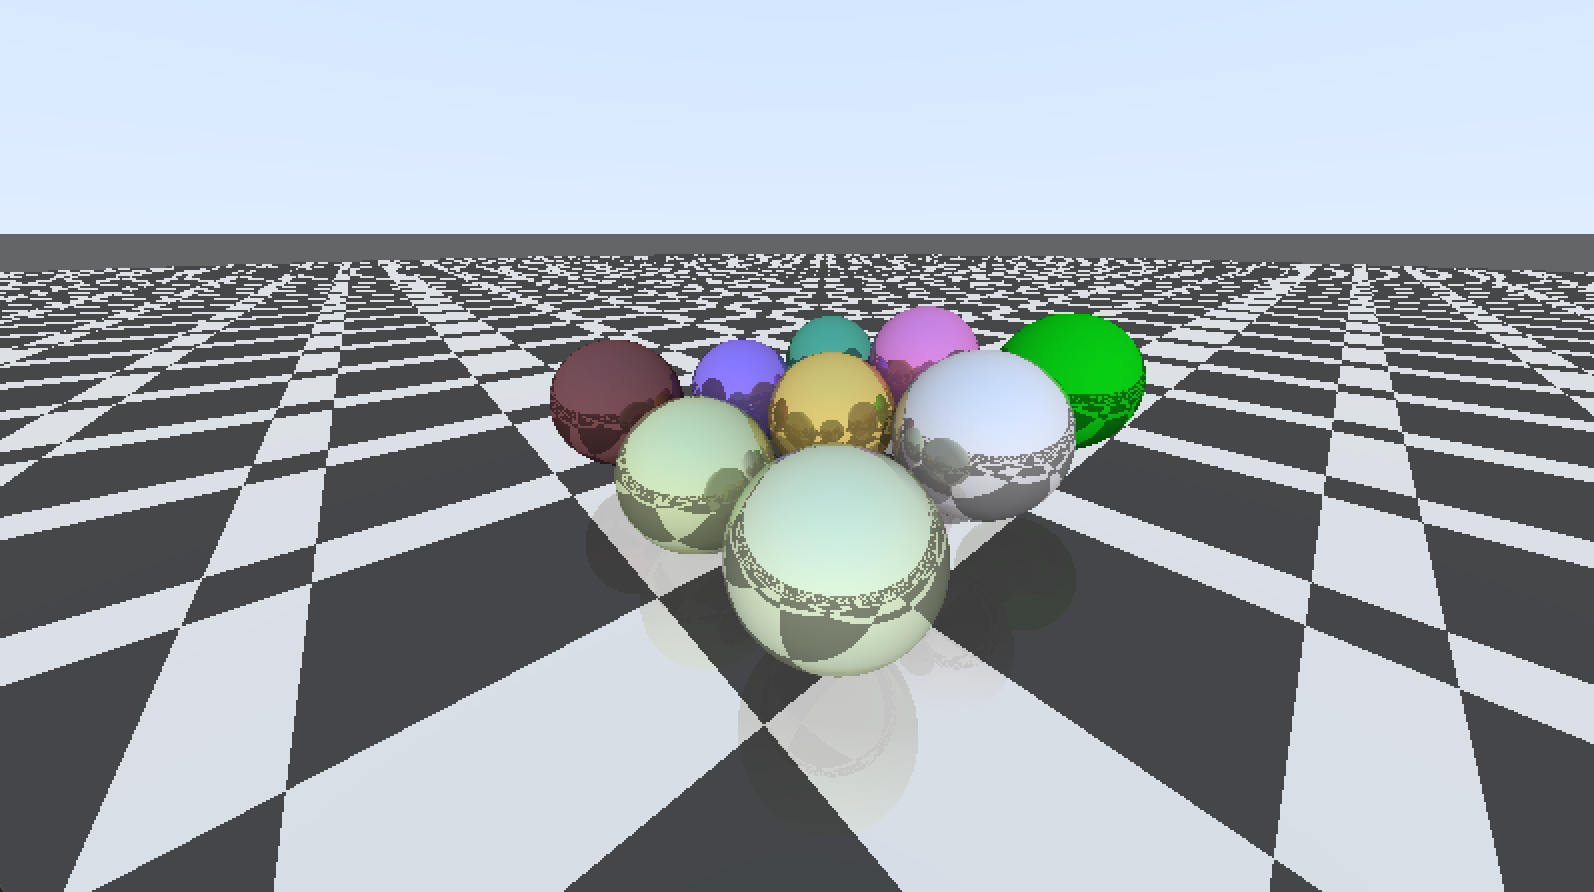
\includegraphics[scale=0.6]{figures/ReflectionDemoScene.png}
    \caption{Demonstration scene highlighting reflections}
    \label{fig:reflect_demo}
\end{figure}
\noindent
If you look closely at the image, particularly the reflections on adjacent spheres, you will notice reflections within the reflections, highlighting the recursive nature of the implementation.
\section{Conclusion}
    Ray tracing is a perfect example of how math can be used to produce detailed, realistic images by modeling processes in the real world. The fairly basic implementation discussed in this article only scratches the surface of what is possible with ray tracing, but the mathematical concepts can be applied throughout computer graphics. Interested readers are encouraged delve deeper into this fascinating rendering technique and try to expand upon this article by implementing features like indirect illumination, fuzzy reflections, refraction, and volumetric rendering which would contribute to a more realistic and complete simulation.
\end{document}
